\chapter{Verification}

\setcounter{section}{6}
\setcounter{subsection}{0}

\subsection{The test application}

To test the framework a test application was written. The test application is a todo-list which allows the user to keep track of what needs to be done. Todo-items can be added, edited, marked as completed and removed. Other features such as clearing all completed tasks and marking all tasks as completed were also implemented. The choice of test application and its features was not randomly picked. The open source project TodoMVC has implemented the exact same application in a wide range of Javascript frameworks \cite{todomvc}. The idea behind the project is to make it easier for developers to compare different Javascript frameworks. It also becomes suitable for verifying MinimaJS since it now can be compared with its competitors. The test application can be seen in figure \ref{fig:testapp}.

\begin{figure}[h!]
	\centerline{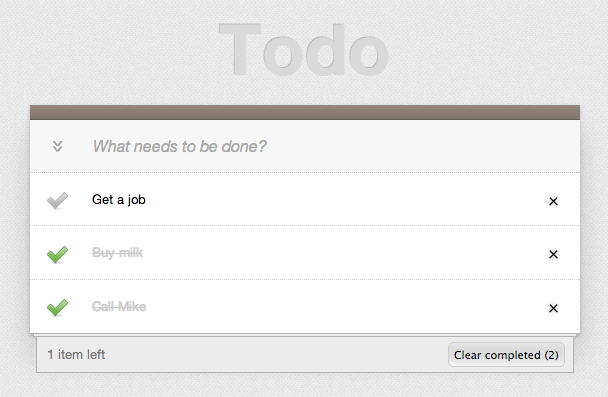
\includegraphics[width=120mm]{gfx/testapp.png}}
	\caption{The test application.}
	\label{fig:testapp}
\end{figure}

\subsection{Measuring the initial loading time}

To see how the framework performed in terms of initial loading time the loading time was measured and compared with implementations in other Javascript frameworks. A comparison was also made against an application that is not depending on Javascript at all, the HTML-files were then simply generated directly by the backend. An implementation written in standard Javascript without any framework at all is also included in the measurements. The files were served through an Apache webserver with the browser running on the same machine as the web server to neglect the transferring time. The transferring time was neglected since focus lies on the performance of the framework and how fast the content can be rendered, not the transferring time itself. The total loading time will always depend on the transferring time but it is of course very dependent on the client. When the measurements were made were there three todo-items in the list, the browser used was Google Chrome 22. Local storage from the HTML5 draft was used as data storage for all the measurements. The result from the measurements can be seen in table \ref{table:loading_time}. The result is also illustrated in figure \ref{fig:loading_time}.

\begin{table}[H]
	\begin{center}
		\noindent\makebox[\textwidth]{
		\begin{tabularx}{1.08\textwidth}{ c | >{\centering}m{1.4cm} | >{\centering}m{3cm} | c | c | c}
			\hline
			\textbf{Action} & \textbf{Static HTML}	& \textbf{Javascript \newline(no framework)}	& \textbf{MinimaJS}		& \textbf{Backbone.js}	& \textbf{Ember.js} \\ \hline
			Download page				& 48 ms		& 36 ms 				& 32 ms				& 30 ms					& 38 ms \\
			Download scripts			& 0	ms		& 37 ms 				& 33 ms				& 36 ms					& 51 ms \\
			Parse scripts				& 0	ms		& 31 ms 				& 81 ms				& 85 ms					& 283 ms \\
			Load application			& 0	ms		& 7 ms 					& 7 ms				& 109 ms				& 449 ms \\
			Fetch data					& 0	ms		& 2 ms 					& 5	ms				& 14 ms					& 31 ms \\
			Render page					& 4	ms		& 13 ms 				& 17 ms				& 16 ms					& 172 ms \\ \hline
			\textbf{Total}				& \textbf{52 ms} & \textbf{126 ms}	& \textbf{175 ms}	& \textbf{290 ms} 		& \textbf{1024 ms}
		\end{tabularx}}
		\caption{The loading time of the test application in different implementations.}
		\label{table:loading_time}
	\end{center}
\end{table}

\begin{figure}[H]
	\centerline{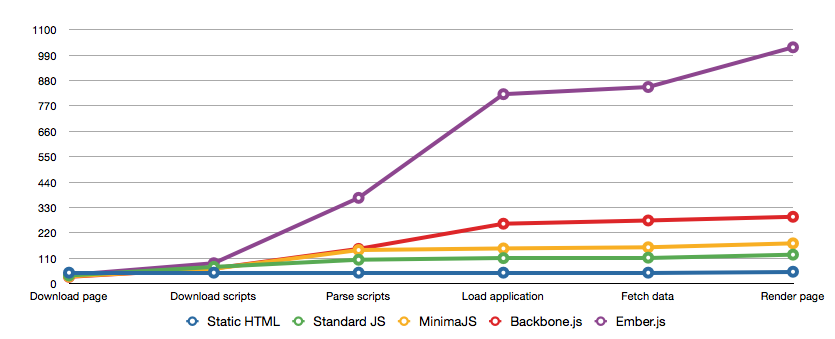
\includegraphics[width=160mm]{gfx/load_time.png}}
	\caption{A graph showing the loading time of the test application comparing different implementations of it.}
	\label{fig:loading_time}
\end{figure}

As expected the page is downloaded faster on all Javascript-based implementation since it is smaller and does not contain the presentation of the all the todo-items. However, the static HTML does not need to download or parse any Javascript which leads to a shorter initial loading time in total. Considering the low transferring time the time it takes to download and parse of the script is still $65\%$ for the MinimaJS framework. This indicates how important it is with a small file size of the framework. Except keeping the size small it hard is affect the total time until the script has completely been loaded and parsed. Also worth noticing is the poor performance of Ember in this test. Since the Ember-implementation is using two-way data-bindings the result is however not very surprising, one of the main drawbacks with two-way data bindings is the loss of performance. In the end all Javascript versions are slower than the static version which confirms Twitter's criticism \cite{twitter_no_hashbang} against SPAs.

Since the size of the framework essentially affects the initial loading time it can be further analyzed. In table \ref{table:frameworks_filesize} is the Javascript frameworks from table \ref{table:loading_time} listed with their respective file size when they have been minified using UglifyJS and compressed with gzip.

\begin{table}[H]
	\begin{center}
		\begin{tabular}{ c | c | c | c }
			\hline
			\textbf{Framework}	& \textbf{Size of framework}	& \textbf{Size of dependencies} & \textbf{Total size} \\ \hline
			MinimaJS 0.1			& 4.3 kB						& 10.4 kB						& 14.7 kB \\
			Backbone.js 0.9.2	& 5.6 kB						& 13.0 kB						& 18.6 kB \\
			%Spine.js 1.0.8		& 6.9 kB						& 13.0 kB						& 19.9 kB \\
			%Angular.js 1.0.1	& 28.7 kB						& 0 kB						 	& 28.7 kB \\
			Ember.js 1.0		& 37.0 kB						& 0 kB						 	& 37.0 kB \\ \hline
		\end{tabular}
		\caption{File size of a few Javascript frameworks after minification and compression.}
		\label{table:frameworks_filesize}
	\end{center}
\end{table}

Note that some of the frameworks in the table have a configurable amount of dependencies. The dependencies are chosen so that the frameworks become as small as possible but still support templates and routing. Underscore was used as template language for MinimaJS and Backbone. While MinimaJS could be configured to use Sizzle as selector library Backbone is depending on Zepto which is a bit bigger. Ember.js have no hard dependencies at all. The size of the frameworks matches the initial load time pretty well, a big framework leads to a long initial loading time. As seen MinimaJS is smaller than both Backbone and Ember, on the other hand is MinimaJS in a very early development phase. The size will most probably increase a bit after bugs have been fixed and the browser support has been improved.

\subsection{Measuring the testability}

To verify the testability a number of unit tests were constructed where each test verified one specific feature in the test application. When these unit tests were executed the code coverage was measured to see how much of the application is used for completing the test. The following features were tested in the test application:

\begin{enumerate}
	\item Add a new todo-item to the list
	\item Read the label of a todo-item from the list
	\item Remove a todo-item from the list
	\item Toggle one todo-item as completed
	\item Set all todo-items as completed
	\item Clear all todo-items from the list that are marked as completed
	\item Change the label of a todo-item in the list
\end{enumerate}

As described in section \ref{sec:background_testing} it is quite messy to write unit tests that make use of the user interface, a better approach is to unit test what is underneath it. The unit tests that were constructed in this test were not allowed to communicate directly with the user interface. When measuring code coverage there are several methods that can be used, in this test was the line coverage measured. The line coverage of an execution represents how many lines of code that were interpreted during the execution, this can be measured in percentage since the total number of lines of code in the application is known. Line coverage not ideal to use in all situations, the number of lines of code does not represent the complexity of the application very well. On the other hand it will give a hint of how much of the application that is being tested. Applications with the exact same functionality were tested for all frameworks. All applications are from the TodoMVC project except the test application for MinimaJS that was implemented in the thesis. 

When running the unit tests the tool JSCoverage was used to measure the line coverage, QUnit was used to run and validate the results from the unit tests. The same type of unit tests were used for all of the frameworks that were tested even though they each had to be tweaked in order to work together with the their respective test-application. One test at a time was run, after running a test the line coverage was measured. As a last test all unit tests were run all together so that the total line coverage could be measured. The result from the testing can be seen in table \ref{table:unit_tests_comparasion}. Features that could not be tested with a unit test without interacting with the user interface were marked with N/A in the table.

\begin{table}[H]
	\begin{center}
		\begin{tabular}{ c | c | c | c | c}
			\hline
			\textbf{Unit test}	& \textbf{Description}			& \textbf{Plain jQuery}	& \textbf{Backbone.js} & \textbf{MinimaJS} \\ \hline
			1 					& Add							& N/A				& 70\%				& 67\%			\\
			2					& Read							& N/A				& 68\%				& 67\%			\\
			3					& Remove						& N/A				& N/A				& 69\%			\\
			4					& Toggle						& N/A				& N/A				& 70\%			\\
			5					& Set all						& N/A				& N/A				& 70\%			\\
			6					& Clear all						& 62\%				& 73\%				& 74\%			\\
			7					& Change label					& N/A				& N/A				& 80\%			\\ \hline
								& \textbf{All tests at once}	& 62\%				& 75\%				& 90\%			
		\end{tabular}
		\caption{A comparison between different frameworks when measuring the line coverage after a unit test was run.}
		\label{table:unit_tests_comparasion}
	\end{center}
\end{table}

As seen in the test result is unit testing not a trivial task when writing Javascript applications, but if the system is designed with testing in mind it is possible to get a high degree of testability. To get 90\% of line coverage without interacting with the UI at all is not too bad for an application written to serve as a user interface. The line coverage becomes in fact quite high already after one single unit test, and this is the case since there typically is a lot of initialization going on like setting up modules and fetching content from the database. The application written in plain jQuery performs quite poor since its components are tightly coupled and DOM elements are passed around between functions which makes them impossible to test without interface with the UI. The problem with the implementation in Backbone is that some of its functionality is hidden behind a function scope which makes its functions impossible to access. In MinimaJS the presentation models are working as a unified interface that the unit tests can communicate with which make all of its features testable.

\subsection{Multiple clients}
In order to test how well the synchronization protocol worked a stress test was constructed. The idea with the stress test was to see if the set of models in each and every client could be kept synchronized even though a large amount of clients were connected and modifying the data on the same server. The test was using the websocket API driver and the server was implemented in Node.js. Even though the same protocol is used for all drivers there are no reason to test the synchronization aspect for the local storage driver since simply there only can be one single client connected at a time. With websockets on the other hand a large number of clients can interact with the database simultaneously.

To construct a proper test each client would be required to run a separate instance of the framework. However, to run and manage hundreds of GUI windows running the framework is not really a practical solution. Instead webworkers in the HTML5 draft were used. The webworker API allows threads to be spawned in the background running a given Javascript-program, the communication with the threads is done through a thread-safe message passing implementation. 

The test program first initialized 100 instances of the framework where each instance was running in a separate thread. When all instances were ready to run a message was sent to them to indicate that they should start their test. The instances then started to do transactions against the database. They randomly picked a valid transaction, either they created a new model or they modified or deleted an existing one. Since all instances were doing their transactions at roughly the same time bursting phenomenons occurred, the server had to handle transactions that lead to conflicts since the same model might have been changed by multiple instances at once. When all instances each had made 10 transactions their version of the data models was sent to the main thread so that they could be compared. If all data from each and every model were the same the test was considered as successful. All instances successfully completed the test and had the same version of their data models.

\subsection{Test of a SEO-friendly Javascript site}

To test the approach of solving the problem with search engine optimizations for Javascript-based sites a test-site was published. The test-site contained four pages with different content. Once the initial page had been loaded the actual content was asynchronously loaded and rendered by Javascript. If the site was loaded in a browser with Javascript turned off a blank white page was returned without any content at all. The solution described in section \ref{sec:seo_a_new_approach} was used to provide the crawler with an HTML-snapshot of the requested page. Once the test-site was submitted to Google the pages could be indexed by Google's crawler. As seen in figure \ref{fig:seotest_result} did Google's crawler successfully indexed all of the four pages. 

\begin{figure}[h!]
	\centerline{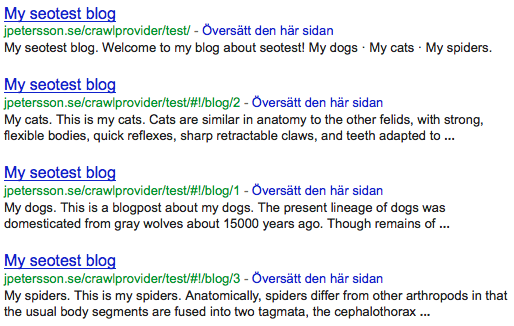
\includegraphics[width=120mm]{gfx/seotest.png}}
	\caption{The result after submitting the test-site to Google's Crawler.}
	\label{fig:seotest_result}
\end{figure}
